\documentclass{article}
\usepackage{graphicx}
\title{Five Programming Languages and Their Origins}
\author{Une Umoh}
\begin{document}
	\maketitle
	\newpage
	
	\title{What are Programming Languages?}
	\maketitle
	
	According to Wikipedia, A programming language is a language comprising of a set of strings that produce various kinds of machine code output. 
	\paragraph{}
	In a simpler way, a programming language can be defined as a language understood by computers consisting of sets of instructions that allow computers carry out tasks
	\newpage
	
	\title{HTML}
	\maketitle
	\begin{figure}
	
\includegraphics[width=\linewidth]{html.jpeg}
		\label{html.01}
	\end{figure}

	\newpage
	HTML stands for Hyper Text Markup Language.It was invented by Sir Tim Berners-Lee in the earlt 90's.
	\paragraph{}
	It wasn't published officially until 1993 for people around the world to share and access information easily.
	\paragraph{}
	It is today one of the most popular programming languages. The latest version of HTML is HTML 5.0. HTML's main purpose is to create websites
	\paragraph{}
	IDEs: Notepad, Notepad++, Brackets, MS FrontPage...
	\paragraph{}
	Related languages: CSS, JavaScript and pHp...
	\newpage
	\title{Java}
	\begin{figure}
		
\includegraphics[width=\linewidth]{java.jpg}
	\end{figure}
	
	\newpage
	The father of Java, James Gosling, invented the language in 1995.
	\paragraph{}
	Java is used for internet programming, mobile devices, creation of games and many more.
	\paragraph{}
	IDEs: BlueJ, Eclipse, Greenfoot etc...
	\paragraph{}
	Related languages: Smalltalk, Lisp, Cypher.
	
	\newpage
	\title{CSS}
	\begin{figure}
		\includegraphics[width=\linewidth]{CSS.jpg}
	\end{figure}

	\newpage
	CSS stands for cascading style sheet and was proposed by Hakon Wium Lei and published in 1966.
	\paragraph{}
	This language was made to add color, layouts, fonts and many other styles to websites.
	\paragraph{}
	IDEs: Netbeans, Komodo edit, Notepad++ etc...
	\paragraph{}
	Related Languages: HTML, SVG, XML etc... 
	
	\newpage
	\title{PhP}
	\begin{figure}	
		
\includegraphics[width=\linewidth]{php.png}
	\end{figure}

	\newpage
	PHP stands for Hyper text preprocessor. It is a scripting language majorly used for web development.
	\paragraph{}
	It was invented by Rasmus Lerdorf, in 1994. The first official release was in 1995.
	\paragraph{}
	IDEs: NetBeans, Eclipse, PhPStorm etc...
	\paragraph{}
	Related Languages: JavaScript, Python, C etc...
	
	\newpage
	\title{JavaScript}
	\begin{figure}	
		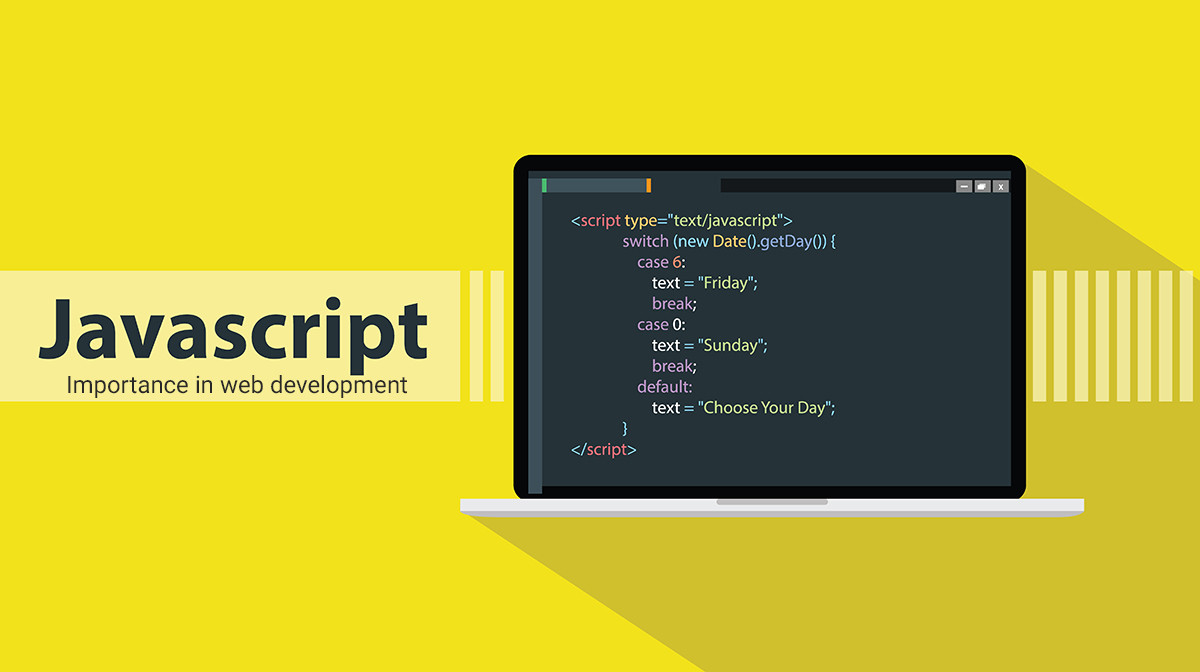
\includegraphics[width=\linewidth]{javascript.jpg}
	\end{figure}
	
	\newpage
\end{document}